\documentclass[10pt,a4paper]{article}

\usepackage[top=2.0cm,bottom=2.2cm,left=2.2cm,right=2.2cm]{geometry}
\usepackage[T1]{fontenc}
\usepackage{lmodern}
\usepackage{microtype}
\usepackage{booktabs}
\usepackage{pgfplots}
\pgfplotsset{compat=1.18}
\usepackage{tikz}
\usetikzlibrary{bending,calc}
\usepackage{xcolor}
\usepackage{parskip}
\usepackage{titlesec}
\usepackage[hidelinks]{hyperref}
\usepackage{caption}
\usepackage{fancyhdr}
\usepackage{lastpage}
\usepackage{array}
\usepackage{float}
\setlength{\headheight}{20pt}
\addtolength{\topmargin}{-8pt}

%% Colours
\definecolor{uoeblue}{RGB}{0,60,113}
\definecolor{midgray}{RGB}{130,130,130}
\definecolor{darkgray}{RGB}{70,70,70}

%% Section style
\titleformat{\section}
  {\normalfont\large\bfseries\color{uoeblue}}{}
  {0em}{}
  [\vspace{-3pt}{\color{uoeblue}\rule{\linewidth}{0.6pt}}]
\titlespacing*{\section}{0pt}{9pt}{4pt}

%% Subsection style (used for result sub-headings)
\titleformat{\subsection}
  {\normalfont\normalsize\bfseries\itshape\color{darkgray}}{}
  {0em}{}
\titlespacing*{\subsection}{0pt}{5pt}{1pt}

\captionsetup{font=small, labelfont=bf, skip=3pt}
\setlength{\parindent}{0pt}
\setlength{\parskip}{4.5pt}

\pagestyle{fancy}
\fancyhf{}
\cfoot{\small\textcolor{midgray}{\thepage\,/\,\pageref{LastPage}}}
\renewcommand{\headrulewidth}{0pt}

\begin{document}

%% ─── Title ──────────────────────────────────────────────────────────────────
\vspace*{-0.3em}
\begin{center}
  {\LARGE\bfseries\color{uoeblue}InfraQ}\\[5pt]
  {\large A Scheduling Gateway for Shared Local LLM Inference}
\end{center}
{\color{uoeblue}\rule{\linewidth}{1.0pt}}
\vspace{3pt}

\textit{InfraQ brings continuous batching and prefix caching, the scheduling techniques
behind vLLM and SGLang, to a Mac~M1 inference stack via RabbitMQ, Redis, and a Python
asyncio worker, without CUDA.
On repeated-prompt workloads, cache-aware dispatching achieved
\textbf{5.6$\times$ higher throughput} and \textbf{76\% lower average latency}
over non-cached strategies; on unique-prompt workloads, continuous dispatching reduced
P95 tail latency by 3\% over static batching by eliminating batch-boundary stalls.}

\vspace{2pt}

%% ─── 1. Problem and Idea ────────────────────────────────────────────────────
\section{Problem and Idea}

Small engineering teams increasingly run shared local LLMs on a Mac server rather than
routing queries to cloud APIs. The problems are predictable: concurrent requests pile
up with no queue, repeated prompts get re-inferred from scratch every time, and there
is no built-in way to compare scheduling choices.

vLLM~\cite{vllm} and SGLang~\cite{sglang} solve these problems at the GPU kernel level:
continuous batching avoids batch-boundary idle time, and prefix caching reuses KV tensors
across shared prompt prefixes. Both require NVIDIA hardware and CUDA toolchains that
most small teams cannot justify.

InfraQ re-implements both techniques at the infrastructure layer, so they work on any
machine running Ollama~\cite{ollama}, including Mac~M1. Teams sharing a local LLM get
lower latency under load, fewer redundant inferences, and a reproducible way to compare
scheduling choices on their own workload.

%% ─── 2. Scheduling Strategies ───────────────────────────────────────────────
\section{Scheduling Strategies}

InfraQ implements four strategies: a sequential baseline, static batching, continuous
dispatching, and cache-aware dispatching. Each builds on the previous one and introduces
exactly one new mechanism, so the experiments in §4 can attribute any performance change
to that mechanism alone. Table~\ref{tab:strategies} summarises them.

\begin{table}[h]
\centering
\caption{The four scheduling strategies in InfraQ.}
\label{tab:strategies}
\small\setlength{\tabcolsep}{5pt}
\renewcommand{\arraystretch}{1.25}
\begin{tabular}{lp{4.0cm}p{2.2cm}p{4.0cm}}
\toprule
Strategy & Mechanism & Inspiration & Trade-off addressed \\
\midrule
Sequential &
  One request at a time; no parallelism &
  Baseline &
  None --- performance floor \\
Static batching &
  Collect $N$ requests; dispatch all; wait for the entire batch to finish &
  Classic GPU batching &
  Gains concurrency, but the slowest request stalls completed slots \\
Continuous dispatching &
  Maintain $K$ slots; refill immediately when any slot completes &
  vLLM continuous batching &
  Eliminates batch-boundary stalls; keeps slots filled \\
Cache-aware dispatching &
  Redis lookup before each slot acquisition; SHA-256 key on model~+~prompt;
  hits return in $\sim$11\,ms, skipping Ollama &
  SGLang prefix caching &
  Near-zero latency for repeated prompts; frees slots for cache misses \\
\bottomrule
\end{tabular}
\end{table}

%% ─── 3. Architecture ────────────────────────────────────────────────────────
\section{Architecture}

The gateway (Spring Boot) returns HTTP~202 immediately, writes a record to PostgreSQL,
caches status in Redis, and publishes the job to RabbitMQ. None of these operations
block on inference. The worker (Python asyncio) consumes from RabbitMQ and applies the active
scheduling strategy. Ollama runs natively on the host and is reached from the worker
container via \texttt{host.docker.internal}, so Mac Metal GPU acceleration works without
container passthrough.

\begin{figure}[h]
\centering
\resizebox{\linewidth}{!}{%
\begin{tikzpicture}[
  box/.style ={draw=uoeblue!55, rounded corners=3pt,
               minimum width=1.75cm, minimum height=0.62cm,
               font=\small, fill=uoeblue!8, align=center},
  hbox/.style={draw=uoeblue, rounded corners=3pt,
               minimum width=1.75cm, minimum height=0.62cm,
               font=\small\bfseries, fill=uoeblue!22, align=center},
  arr/.style ={->, >=stealth, thick, color=darkgray},
  darr/.style={->, >=stealth, thick, dashed, color=uoeblue!70},
  lbl/.style ={font=\scriptsize\itshape, color=darkgray}
]
  %% ── Top row: request path (3 cm spacing) ───────────────────────────────
  \node[hbox] (cli) at (0,    0)   {Browser};
  \node[box]  (gw)  at (3.0,  0)   {Gateway\\(Spring Boot)};
  \node[box]  (mq)  at (6.0,  0)   {RabbitMQ};
  \node[box]  (wk)  at (9.0,  0)   {Worker\\(asyncio)};
  \node[hbox] (ol)  at (12.0, 0)   {Ollama\\(Metal GPU)};

  %% ── Bottom row: storage ─────────────────────────────────────────────────
  \node[box]  (pg)  at (3.0, -1.8) {PostgreSQL};
  \node[box]  (rd)  at (9.0, -1.8) {Redis};

  %% ── Request path (top row, left → right) ────────────────────────────────
  \draw[arr] (cli) -- (gw)  node[lbl,above,midway]{POST};
  \draw[arr] (gw)  -- (mq)  node[lbl,above,midway]{enqueue};
  \draw[arr] (mq)  -- (wk)  node[lbl,above,midway]{consume};
  \draw[arr] (wk)  -- (ol)  node[lbl,above,midway]{infer};

  %% ── Gateway → PostgreSQL (persist) ──────────────────────────────────────
  \draw[arr] (gw) -- (pg) node[lbl,right,midway]{persist};

  %% ── Worker ↔ Redis: two parallel vertical arrows, offset ±0.12 cm ───────
  \draw[arr]  ($(wk.south)+( 0.12,0)$) -- ($(rd.north)+( 0.12,0)$)
    node[lbl,right,midway]{result};
  \draw[darr] ($(rd.north)+(-0.12,0)$) -- ($(wk.south)+(-0.12,0)$)
    node[lbl,left, midway]{config};

  %% ── Redis → Gateway (state / cache): diagonal ───────────────────────────
  \draw[arr] (rd) -- (gw) node[lbl,above,midway,sloped]{state\,/\,cache};

\end{tikzpicture}%
}
\caption{InfraQ system architecture. The top row shows the synchronous request path;
the bottom row shows persistent storage and the inference engine.
The dashed arrow is the Redis configuration channel through which live strategy
changes propagate from the gateway to the worker.}
\label{fig:arch}
\end{figure}

Redis serves four roles: browser-polling fast-path ($<$1\,ms), prompt-result cache,
atomic metric counters, and the live configuration channel shown dashed in
Figure~\ref{fig:arch}.
PostgreSQL stores permanent records (full request histories and per-request timing)
for offline analysis.
On a configuration change, the worker drains all in-flight tasks then restarts under
the new strategy without container restarts.

%% ─── 4. Experimental Results ────────────────────────────────────────────────
\section{Experimental Results}

MacBook Air M1 (8\,GB), Qwen2.5:1.5b via Ollama; 100~requests per run, 5~repeats.
Unique runs used 100 distinct prompts (40 topics $\times$ 4 templates, no repeats).
Repeated runs cycled an 8-prompt hot set for 80\% of requests and inserted unique
prompts for the remaining 20\%, yielding an average 71\% cache hit rate.
Raw data are in \texttt{summary.csv} and \texttt{manifest.json} in the submission.

\subsection*{Scheduling without caching (unique prompts)}

\begin{table}[H]
\centering
\caption{Experiment A --- unique prompts (no cache benefit). 5-run averages.}
\label{tab:expa}
\small\setlength{\tabcolsep}{7pt}
\begin{tabular}{lcrrr}
\toprule
Strategy        & Slots & Avg latency & P95     & Throughput   \\
\midrule
Sequential      & 1     & 188\,s      & 442\,s  & 0.213\,req/s \\
Static batching & 8     & 185\,s      & 438\,s  & 0.213\,req/s \\
Continuous      & 8     & 180\,s      & \textbf{426\,s} & \textbf{0.219\,req/s} \\
Cached          & 8     & 179\,s      & 430\,s  & 0.218\,req/s \\
\bottomrule
\end{tabular}
\end{table}

\begin{figure}[H]
\centering
\begin{tikzpicture}
\begin{axis}[
  xbar,
  width=0.76\linewidth, height=4.2cm,
  xmin=0.195, xmax=0.225,
  xlabel={Throughput (req/s)},
  ytick={0,1,2,3},
  yticklabels={Sequential 1sl, Static 8sl, Continuous 8sl, Cached 8sl},
  ymin=-0.6, ymax=3.6,
  nodes near coords,
  nodes near coords align={horizontal},
  every node near coord/.style={font=\small},
  bar width=10pt,
  tick label style={font=\small},
  xlabel style={font=\small},
  xmajorgrids=true,
  grid style={dashed, gray!25},
  axis line style={midgray},
  tick style={midgray},
]
\addplot[fill=uoeblue!70, draw=uoeblue!90] coordinates {
  (0.213,0) (0.213,1) (0.219,2) (0.218,3)
};
\end{axis}
\end{tikzpicture}
\caption{Throughput on the unique-prompt workload (Experiment~A). Differences between
strategies are small ($\le$3\%) because all four share the same Ollama token-generation
ceiling; continuous dispatching still edges the others by avoiding batch-boundary stalls.}
\label{fig:expa}
\end{figure}

With every prompt unique the cache cannot fire, so the numbers isolate the scheduling
mechanism. Continuous dispatching beats static batching on throughput by 2.8\%
(0.219 vs.\ 0.213\,req/s) and on P95 tail latency by 2.7\% (426\,s vs.\ 438\,s),
consistently across all five repeats. Static batching waits for the slowest request in
a batch before refilling any freed slot; continuous dispatching refills the moment a
slot frees.

\subsection*{Cache-aware dispatching on repeated prompts}

\begin{table}[H]
\centering
\caption{Experiment B --- repeated prompts (hot prompt set). 5-run averages.}
\label{tab:expb}
\small\setlength{\tabcolsep}{6pt}
\begin{tabular}{lcrrrr}
\toprule
Strategy          & Slots & Avg latency & P95     & Throughput   & Hit rate \\
\midrule
Sequential        & 1     & 311\,s      & 584\,s  & 0.165\,req/s & 0\%  \\
Static batching   & 4     & 298\,s      & 557\,s  & 0.173\,req/s & 0\%  \\
Continuous        & 4     & 299\,s      & 565\,s  & 0.170\,req/s & 0\%  \\
\bfseries Cached  & \bfseries 4 & \bfseries 73\,s &
\bfseries 96\,s & \bfseries 0.961\,req/s & \bfseries 71\% \\
\bottomrule
\end{tabular}
\end{table}

With 71\% of requests hitting the cache, cache-aware dispatching delivers a
5.6$\times$ throughput increase (0.961 vs.\ 0.170\,req/s) and reduces average latency
by 76\% (73\,s vs.\ 299\,s) over non-cached continuous dispatching. Each cache hit
returns in $\sim$11\,ms rather than the $\sim$300\,s average inference time, a per-hit
saving of 96.3\%. With only 29 requests per 100 reaching Ollama, slots stay freer and
P95 tail latency collapses from $\sim$565\,s to 96\,s (83\% reduction).

\subsection*{Slot-count ablation (cached strategy)}

Increasing the slot count from 4 to 8 under cache-aware dispatching actually
\textit{reduces} performance: throughput falls from 0.961 to 0.699\,req/s and the hit
rate drops from 71\% to 67\%. The cache starts cold, so the first wave of requests are
all misses. With 8 slots, 8 simultaneous misses hit Ollama before any result is written
back to Redis; with 4 slots, fewer misses compete for Ollama's capacity and hits
accumulate sooner. For cache-aware scheduling, the optimal slot count depends on
workload repetition rate and cache warm-up. More concurrency is not always better.

%% ─── 5. Implementation ──────────────────────────────────────────────────────
\section{Implementation}

All four strategies are implemented, tested, and live-switchable without container
restarts. Deployment is a single \texttt{docker compose up}; the only external dependency
is Ollama with the target model loaded. The web interface exposes a chat tab, a live
metrics dashboard, and the benchmark lab that produced the results in §4.

The caching layer is prototype-grade: InfraQ stores exact-match text results rather than
KV tensors, so semantically similar prompts still miss. A production system would replace
this with embedding-based semantic matching.

%% ─── 6. AI Usage ────────────────────────────────────────────────────────────
\section{AI Usage}

All scheduling ideas (continuous batching adapted from vLLM, prefix caching adapted from
SGLang) were conceived by the author. System architecture and experimental methodology
were designed by the author. ChatGPT and Claude Code assisted with writing code; the
web UI was generated by AI from a detailed specification written by the author. This
report was polished with AI assistance, and the architecture diagram was drawn with
AI tooling.

%% ─── References ─────────────────────────────────────────────────────────────
\newpage

{\small
\begin{thebibliography}{[9]}
\setlength{\itemsep}{4pt}
\setlength{\parsep}{0pt}

\bibitem{vllm}
W.~Kwon, Z.~Li, S.~Zhuang, Y.~Sheng, L.~Zheng, C.~H.~Yu, J.~E.~Gonzalez, H.~Zhang,
and I.~Stoica, ``Efficient memory management for large language model serving with
PagedAttention,'' in \textit{Proc.\ 29th ACM Symposium on Operating Systems Principles
(SOSP~'23)}, 2023, pp.~611--626.

\bibitem{sglang}
L.~Zheng, L.~Yin, Z.~Xie, C.~Sun, J.~Huang, C.~H.~Yu, S.~Cao, C.~Kozyrakis, I.~Stoica,
J.~E.~Gonzalez, C.~Barrett, and Y.~Sheng, ``SGLang: Efficient execution of structured
language model programs,'' in \textit{Advances in Neural Information Processing
Systems 37 (NeurIPS 2024)}, 2024.

\bibitem{ollama}
Ollama, ``Get up and running with large language models locally,''
\url{https://ollama.com}, accessed April 2026.

\end{thebibliography}
}

\end{document}
